% Control Objectives Illustration
% TikZ diagram for Chapter 1

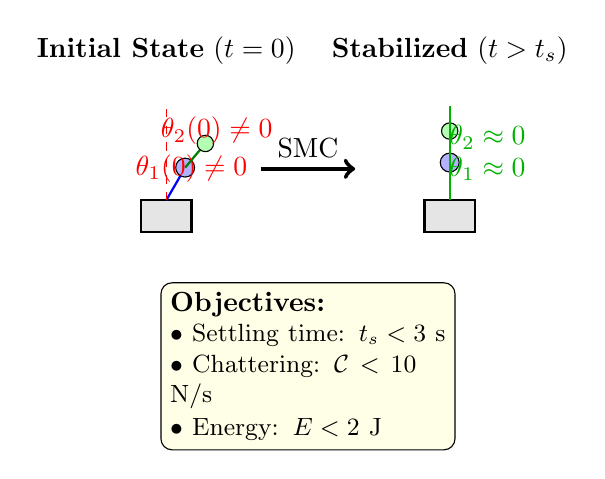
\begin{tikzpicture}[scale=0.8]
    % Initial state
    \begin{scope}
        \node[above] at (0, 2.5) {\textbf{Initial State} ($t=0$)};

        % Cart
        \draw[thick, fill=gray!20] (-0.4, 0) rectangle (0.4, 0.5);

        % Pendula (perturbed)
        \draw[thick, blue] (0, 0.5) -- ({0.6*sin(30)}, {0.5 + 0.6*cos(30)});
        \draw[fill=blue!30] ({0.6*sin(30)}, {0.5 + 0.6*cos(30)}) circle (0.15);

        \draw[thick, green!50!black] ({0.6*sin(30)}, {0.5 + 0.6*cos(30)}) --
                                     ({0.6*sin(30) + 0.5*sin(40)}, {0.5 + 0.6*cos(30) + 0.5*cos(40)});
        \draw[fill=green!30] ({0.6*sin(30) + 0.5*sin(40)}, {0.5 + 0.6*cos(30) + 0.5*cos(40)}) circle (0.13);

        % Reference vertical
        \draw[dashed, red] (0, 0.5) -- (0, 2);

        % Angles
        \node[red] at (0.4, 1.0) {$\theta_1(0) \neq 0$};
        \node[red] at (0.8, 1.6) {$\theta_2(0) \neq 0$};
    \end{scope}

    % Arrow
    \draw[->, ultra thick] (1.5, 1) -- (3, 1) node[midway, above] {SMC};

    % Final state (stabilized)
    \begin{scope}[xshift=4.5cm]
        \node[above] at (0, 2.5) {\textbf{Stabilized} ($t > t_s$)};

        % Cart
        \draw[thick, fill=gray!20] (-0.4, 0) rectangle (0.4, 0.5);

        % Pendula (upright)
        \draw[thick, blue] (0, 0.5) -- (0, 1.1);
        \draw[fill=blue!30] (0, 1.1) circle (0.15);

        \draw[thick, green!50!black] (0, 1.1) -- (0, 1.6);
        \draw[fill=green!30] (0, 1.6) circle (0.13);

        % Reference vertical (overlapping)
        \draw[thick, green!70!black] (0, 0.5) -- (0, 2);

        % Check marks
        \node[green!70!black] at (0.6, 1.0) {$\theta_1 \approx 0$ \checkmark};
        \node[green!70!black] at (0.6, 1.5) {$\theta_2 \approx 0$ \checkmark};
    \end{scope}

    % Performance metrics
    \node[below, align=left, draw, rounded corners, fill=yellow!10, text width=3.5cm] at (2.25, -0.8) {
        \textbf{Objectives:}\\
        \small
        $\bullet$ Settling time: $t_s < 3$ s\\
        $\bullet$ Chattering: $\mathcal{C} < 10$ N/s\\
        $\bullet$ Energy: $E < 2$ J
    };

\end{tikzpicture}
